\section{Quasipolynomial improvements}
\label{sec:quasipolynomial}

The construction has two steps. First, a dynamic program chooses one
block order satisfying a logarithmic number of nested deadlines, or
minimizing the corresponding weighted delay. Combined with the
supporting-prefix and endpoint lemmas, this gives a legal baseline tree
with cost $2\lambda\OPT$ plus a logarithmic or entropy penalty, where
$\lambda>1$ is the grade spacing. Second, exact optimization of a
logarithmic-depth initial tree removes that penalty. Together these
steps give $(2+\varepsilon)$ approximations for both objectives.
Every query remains a supplied line. Optimal witness paths occur only
in the analysis: the algorithms use interval demands, actual child
costs, and the supplied prior.

\subsection{Nested interval deadlines}

Algorithm~\ref{alg:grade-dp} gives the shared DP; Algorithm~\ref{alg:qp-baselines}
uses it in the two recursions, and Algorithm~\ref{alg:rollout} performs
the exact initial-tree optimization.

Let $M$ candidates be in linear spatial order, and suppose interval
demands have deadlines among $b_1<\cdots<b_r$. A selected candidate is
assigned a grade $i\in[r]$. Scan positions from left to right and store
for each grade prefix $j$ its selected count $c_j$ and last selected
position $p_j$ (zero if none). Selecting position $q$ at grade $i$
increments $c_j$ and sets $p_j=q$ for every $j\ge i$; skip is the
other transition. Reject if $c_j>b_j$. When $[l,q]$ of deadline
$b_j$ ends, require $p_j\ge l$. The invariant is that these are
exactly the count and rightmost selected position among scanned
candidates of grade at most $j$. Thus the interval check is equivalent
to having a qualifying selected point in that demand.

Listing selected candidates in grade order yields a schedule: each
deadline-$b_j$ demand is met in its grade prefix, whose length
$c_j\le b_j$. Conversely, give each query in any feasible schedule
the first deadline bucket at least its rank and discard queries after
all deadlines. This maps every feasible schedule to a DP witness, so
the test is exact. There are at most $(M+1)^r(B+1)^r$ states for
$B=\max b_j$, with $r+1$ transitions per position. For circular
demands, enumerate the first candidate $v$, remove demands containing
it, and cut there. Its forced rank-one query consumes one unit in
\emph{every} cumulative count, so residual capacities are $b_j-1$.

Independent coverage at each deadline need not be jointly feasible.
On candidates $1,2,3$, let $[1,2]$ and $[2,3]$ have deadline one,
and let $\{1\}$ and $\{3\}$ have deadline two. Each prefix is
separately coverable, but no ordering works: 2 must be first, and then
both 1 and 3 are needed by rank two. The grade-vector DP captures this
nesting constraint.

\begin{algorithm}[H]
\caption{\GradeDP: cumulative-grade interval feasibility or weighted delay}
\label{alg:grade-dp}
\KwIn{Ordinary intervals; capacities $b_0<\cdots<b_r$;
feasibility deadlines, or weights and delay levels $d_j=b_j-1$.}
\KwOut{A feasible graded selection, or a minimum surrogate-delay selection.}
Initialize the state $(c_0,\ldots,c_r;s_0,\ldots,s_r)$ to all zeros,
with cost zero; all other states are unreachable\;
\For{$q=1,\ldots,M$}{
  From each reachable state, try skipping $q$ or selecting it at grade $i$\;
  A grade-$i$ selection increments $c_j$ and sets $s_j=q$ for all $j\ge i$\;
  Reject any transition with $c_j>b_j$\;
  \ForEach{interval $I=[l,q]$ ending here}{
    \eIf{mode is feasibility}{
      Reject if $s_j<l$ for its deadline grade $j$\;
    }{
      Find the least $j$ with $s_j\ge l$; reject if none\;
      Add $2w(I)d_j$ to this transition's cost\;
    }
  }
  Keep one feasible witness, or the minimum cost, for each resulting state\;
}
In weighted mode add $2p_0c_r$ to each final state's cost\;
Reconstruct a winning selection and order it by grade\;
\KwRet the selection and schedule, or infeasible\;
\end{algorithm}

For circular demands enumerate the forced first candidate, remove
its demands, cut there, and reduce \emph{every} capacity by one.
Residual expected costs still use the original delay levels and add
$2p_0(1+c_r)$ at completion. In maximum-depth mode append a final
grade with the total-count cap if it is not already a capacity.
Section~\ref{sec:quasipolynomial} proves the state invariant and
the $(M+1)^{O(r)}(B+1)^{O(r)}$ bound.


\subsection{Adjacent support blocks and shifted delays}

Use the edges of the full normalized hull, including the origin if
it is a hull vertex, as candidate \emph{blocks}. Within a block,
query its real endpoints in a fixed order, skipping cached answers;
the origin is a free known-negative marker and is never queried.
A positive vertex interval meets a consecutive circular interval of
edges, obtained by including its incident edges. Thus the block-hit
demands are circular intervals too. A two-support original query
maps to its supporting edge; a singleton support maps to any incident
edge. This can only make a class get hit earlier. Repeated or
unproductive blocks may be deleted. In dimension at most one, the
at most two real vertices determine the pattern directly, and the
same upper bounds apply.

Write $k$ for the first hitting block's rank and
$z_A=\lfloor\log_2(\delta s/|A|)\rfloor$ in a count-flat state.
If the first queried endpoint is positive, discovery and endpoint
recovery cost at most $2k-1+z_A+4$.
If the second endpoint is the first positive answer, its adjacent
endpoint is known negative, so the cost is at most $2k+z_A+2$.
A block with just one real endpoint costs at most $2k-1+z_A+4$.
Consequently all routes obey
\begin{equation}\label{eq:qp-block-allowance}
 \text{discovery plus endpoint cost for }A\ \le 2(k-1)+z_A+5.
\end{equation}
For expected depth the same accounting gives an overhead of at most
five per unit of nonzero-pattern mass, in addition to the residual
pattern entropy. Pairing the queries preserves the saving from the
negative first endpoint on a second-endpoint exit.

\begin{algorithm}[H]
\caption{Graded adjacent-block recursion: the quasipolynomial baselines}
\label{alg:qp-baselines}
\KwIn{State $S$; objective $o$; rational $\lambda>1$ and the associated balance parameters.}
\KwOut{The baseline tree of Section~\ref{sec:quasipolynomial}.}
Stop at a singleton; at a balanced state query a balanced line and recurse\;
At a flat state compute $\HullData(S)$ and use full-hull edges as blocks\;
Handle a hull of dimension at most one by its direct extreme tests\;
\eIf{$o=\mathrm W$}{
  Build the pattern children once and record their heights $C_W(A)$\;
  \For{trial heights $H$ in increasing order}{
    Compute $B_A=\lfloor(H-C_W(A)-z_A-5)/2\rfloor$; reject negative budgets\;
    Round each down to the last level in $\{0\}\cup\{\lfloor\lambda^j\rfloor\}$ not exceeding it\;
    Use deadlines $\widehat B_A+1$ and total cap $\lfloor H/2\rfloor$
    in circular $\GradeDP$; stop at the first feasible trial\;
  }
}{
  Use distinct levels $d_0=0$, $d_j=\lfloor\lambda^j\rfloor$ through a level covering $n$\;
  Minimize the circular weighted-delay surrogate with capacities $d_j+1$
  by $\GradeDP$ and zero-pattern mass $w(A_0)$\;
}
Execute the selected blocks, use pointwise endpoint codes for $\mathrm W$
or expected endpoint codes for $\mathrm E$, and attach recursive pattern children\;
Identify the zero singleton after the negative cover if present; omit it otherwise\;
\KwRet the contracted tree\;
\end{algorithm}

The maximum-depth trial range is
$1\le H\le\lceil(2\lambda+\gamma)(|S|-1)\rceil$.
No optimum value or comparison witness is an algorithm input.


\subsection{Maximum depth}

Fix rational $\lambda>1$, $a=2\lambda$, and rational
$0<\delta<1/3$, $\gamma\ge1$ satisfying
\begin{equation}\label{eq:qp-max-parameters}
 \gamma\log_2\frac1{1-\delta}\ge1,\qquad
 \gamma\log_2\frac1\delta\ge5.
\end{equation}
The algorithm constructs a tree satisfying
\begin{equation}\label{eq:qp-max-induction}
 C_W(S)\le\left\lfloor a\OPT_W(S)+\gamma\log_2|S|\right\rfloor.
\end{equation}
At a flat state, first construct all pattern-child codes and record
their actual heights $C_W(A)$. Enumerate a trial height $H$ and a
forced first block. For each nonzero class set the integer delay budget
\[
 B_A=\left\lfloor\frac{H-C_W(A)-z_A-5}{2}\right\rfloor.
\]
Reject negative budgets. Round each $B_A$ down to the largest level
$\widehat B_A$ in $\{0\}\cup\{\lfloor\lambda^j\rfloor:j\ge0\}$
not exceeding it, and give the class the block-rank deadline
$\widehat B_A+1$. Demands hit by the first block are removed; its
rank consumes one unit of every prefix capacity, so remaining
capacities are $\widehat B_A$. Cut the circular block order there
and use the nested interval-deadline DP. Also cap the total selected
block count, including the forced block, at $\lfloor H/2\rfloor$.
Order the selected blocks by grade, execute them, and attach the
endpoint exits and child codes. The all-negative route stops after
all nonzero patterns are covered and identifies the zero singleton,
if present. Trials need only reach
$\lceil(a+\gamma)(|S|-1)\rceil$.

To prove the induction, put $s=|S|$, $D=\OPT_W(S)$,
$x=\log_2(s/|A|)$, $L=\log_2(1/\delta)$, and let $t=t_A$ be the
supporting-prefix index. Restriction gives
$\OPT_W(A)\le D-(t-1)$. At
$H^*=\lfloor aD+\gamma\log_2s\rfloor$, the integer
$E_A=H^*-C_W(A)-z_A-5$ satisfies
\begin{align*}
 E_A&\ge\lfloor a(t-1)+\gamma x\rfloor-\lfloor x-L\rfloor-5\\
 &\ge\lfloor a(t-1)+(\gamma-1)x+L\rfloor-5\\
 &\ge\lfloor a(t-1)+\gamma L\rfloor-5
 \ge\lfloor a(t-1)\rfloor.
\end{align*}
Here $x>L$, $\gamma\ge1$, and \eqref{eq:qp-max-parameters} were
used. It follows that
\[
 B_A\ge\left\lfloor\frac{\lfloor2\lambda(t-1)\rfloor}{2}\right\rfloor
 =\lfloor\lambda(t-1)\rfloor.
\]
For $t=1$ the zero delay level suffices. Otherwise, if
$\widehat B_A=\lfloor\lambda^j\rfloor$, choose $j$ as the last
exponent with $\lfloor\lambda^j\rfloor\le B_A$, including any
duplicate-floor plateau. Maximality then gives
$\lambda^{j+1}\ge B_A+1>\lambda(t-1)$, hence
$\widehat B_A\ge t-1$. This downward rounding retains the exact
integer credit; rounding a real expression first would not suffice.

Map the optimal witness path into its supporting blocks. Every
class is hit by block rank at most $t_A$, and therefore meets its
deadline. If the path terminates at an uncovered nonzero singleton,
append an incident block hitting it; its supporting-prefix index
is $q+1$. The block count is at most $D$ when the zero pattern is
present and at most $D+1$ otherwise. The constraints imply
$\gamma>2$: for $\delta\le1/4$ the first parameter inequality
gives $\gamma\ge1/\log_2(4/3)>2$, while for $\delta>1/4$
the second gives $\gamma>5/2$. Hence for $s\ge2$,
$\lfloor H^*/2\rfloor\ge D+1$. Thus the comparison fits the total
count cap. Enumerating its first block proves trial $H^*$ feasible.
Equation~\eqref{eq:qp-block-allowance} then bounds every positive
exit by $H^*$; the zero route costs at most $H^*$ as well.
Balanced states use the same one-query count-potential argument,
completing the induction.

Since $D\ge\log_2s$, the direct factor is at most $a+\gamma$.
Use the manuscript's rational maximum-depth parameters
$\delta=245122334/10^9$ and $\gamma=246496526/10^8$.
For $\lambda=10000001/10000000$ this gives
\[
 a+\gamma=4.46496546<4.464966.
\]
The less fine grading $\lambda=2001/2000$ gives a factor below $4.466$.
The limiting bound is approximately $4.46496526$, at the solution of
$\delta=(1-\delta)^5$. The rational inequalities are certified by
the logarithm series in \eqref{eq:rational-log-bounds}.
There are $O(\log n/(\lambda-1))$ grades, with polynomially bounded
counts and last positions. The state space and total running time
are $(mn)^{O(\log n/(\lambda-1))}$ for fixed parameters, with
rational arithmetic of polynomial bit length.

\subsection{Arbitrary-prior expected depth}

For positive block demands $I$ of weights $w(I)$ and zero-pattern
mass $p_0\ge0$, minimize over block orders $Q$
\[
 F(Q)=2\sum_I w(I)(\operatorname{first}_Q(I)-1)+2p_0|Q|.
\]
An optimum uses at most the number of demands, since unproductive
blocks can be deleted. Use delay level $d_0=0$ and distinct positive
levels $d_j=\lfloor\lambda^j\rfloor$ through a level covering $n$.
The spatial DP stores grade-prefix last positions $p_j$ and counts
$c_j\le d_j+1$. When interval $[l,q]$ ends,
let $\tau(I)$ be the least $j$ with $p_j\ge l$; reject if none exists
and charge $2w(I)d_{\tau(I)}$. Keep the least accumulated cost per
state and add $2p_0c_{\rm last}$ at completion. Each interval is
charged once at its right endpoint, and $\tau(I)$ is its earliest
selected grade. Ordering selected blocks by grade gives actual hit
delay at most $d_{\tau(I)}$ and length exactly $c_{\rm last}$.

Rank $k=1$ has delay zero and uses grade zero. For $k\ge2$, the
first positive level at least $k-1$ satisfies $d_j<\lambda(k-1)$.
Assigning comparison-order
blocks to these grades respects every capacity $d_j+1$. Thus the
minimum surrogate is at most $\lambda$ times the positive delay
cost plus the unchanged zero waiting cost, and hence at most
$\lambda F(Q)$ for any comparison $Q$. For circular demands
enumerate the first block, remove demands containing it at charge
zero, and cut there. Reduce every cumulative capacity by one and add
$2p_0(1+c_{\rm last})$. Enumerating the comparison's first block
and assigning its remaining blocks by their absolute ranks proves
the same guarantee.
This exact optimization DP has quasipolynomial
$(mn)^{O(\log n/(\lambda-1))}$ running time and polynomial-bit rational
arithmetic.

To bound the comparison ordering, let
$D_+=\sum_{A\ne A_0}w(A)(t_A-1)$ and
$b=\sum_{A\ne A_0}w(A)$. The supporting-block witness order hits
each class by block rank $t_A$. An uncovered terminal nonzero
singleton can be hit by appending an incident block. If $A_0$
exists, the number of blocks is at most the witness path length $q$;
the supporting-prefix lemma gives
$D_++w(A_0)q\le\Delta_{\mathrm E}(S,\Pi)$. The cover-order guarantee
therefore bounds the selected schedule's delay and zero waiting
cost by $2\lambda\Delta_{\mathrm E}$. If $A_0$ is absent, the
appended singleton is covered by its index $t=q+1$ and there is
no zero waiting term.

Write $I=I(S,\Pi)$ for full-pattern information and $J$ for the
discovery-transcript information. The first-endpoint exits have
discovery cost at most $2(k-1)+1$ and endpoint overhead four;
second-endpoint exits have discovery cost at most $2(k-1)+2$ and
overhead two because their neighbor is known negative. Thus
\[
 W_{\rm stage}\le2\lambda\Delta_{\mathrm E}
 +5b+(I-J)/\ln2.
\]
The actual vertex-answer transcript is used for $J$, so every
nonzero discovery cell still lies in one cap of mass below $\delta$,
even though a block can meet the union of two caps.
In a flat state, the capped-discovery lemma gives $J\ge b\sigma(\delta)$,
where
\[
 h(\delta)=-\delta\ln\delta-(1-\delta)\ln(1-\delta),\quad
 k=\lfloor1/\delta\rfloor,\quad r=1-k\delta,\quad
 \sigma(\delta)=-k\delta\ln\delta-r\ln r,
\]
and $0\ln0=0$. Put
\[
 c=\max\{1/h(\delta),\ 5/\sigma(\delta),\ 1/\ln2\}.
\]
Apply Lemma~\ref{lem:stage-conversion} with $A=2\lambda$ and
$B=5$. It pays for endpoint overhead from the discovery information,
then telescopes the remaining restriction and entropy terms. Thus
\begin{equation}\label{eq:qp-expected-ratio}
 C_{\mathrm E}(S)\le2\lambda\OPT_{\mathrm E}(S)+c\mathcal E(S),\qquad
 R\le2\lambda+\max\left\{\frac{\ln2}{h(\delta)},
 \frac{5\ln2}{\sigma(\delta)},1\right\}.
\end{equation}
There is no subtraction of one from the endpoint coefficient because
the remaining pattern entropy still has to be paid.

Take $\lambda=100001/100000$ and $\delta=139087/10^6$. For an exact
certificate use the rational logarithm bounds to verify
\[
 (42967/25000)h(\delta)>\ln2,\qquad
 (42967/25000)\sigma(\delta)>5\ln2.
\]
Thus both terms in the maximum are below $42967/25000=1.71868$, and
\begin{equation}\label{thm:qp-expected}
 C_{\mathrm E}(S)<\frac{37187}{10000}\OPT_{\mathrm E}(S)
 =3.7187\OPT_{\mathrm E}(S).
\end{equation}
As $\lambda\to1$, numerical optimization of this bound approaches
$3.71867512$ near $\delta=0.13908730$; the limit is numerical,
whereas $3.7187$ is the certified bound. The guarantee applies to
arbitrary strictly positive priors and is independent of the smallest
probability.

\subsection{Logarithmic-depth lookahead: factors approaching two}

Algorithm~\ref{alg:rollout} optimizes the first $k$ levels and then
attaches a baseline tree at each surviving state. Its guarantee uses
the same principle for both objectives: each level already paid for
at unit cost replaces a level charged at factor $a>1$ in the baseline.
For maximum depth this saving is pathwise; for expected depth it is
weighted by the mass still on the frontier.

Let $B_W(S)$ and $B_E(S)$ be the actual baseline costs, zero on
singletons. Set $F_0(S)=B_W(S)$ and $G_0(S)=B_E(S)$. For $j\ge1$,
the exact initial-tree recurrences are
\begin{align*}
 F_j(S)&=\min\left\{B_W(S),\;
 1+\min_{\ell\text{ splits }S}\max_{b\in\{0,1\}}F_{j-1}(S_{\ell,b})
 \right\},\\
 G_j(S)&=\min\left\{B_E(S),\;
 w(S)+\min_{\ell\text{ splits }S}
 \bigl(G_{j-1}(S_{\ell,0})+G_{j-1}(S_{\ell,1})\bigr)\right\}.
\end{align*}
The baseline option permits earlier stopping. Queries constant on
$S$ are omitted, and expected costs retain the original prior
weights. Memoizing $(S,j)$ and retaining minimizing choices gives
a legal tree attaining these values. The comparison tree in the
next lemma establishes an upper bound; it is never an input to the
recurrences.

\begin{lemma}[Lookahead removes bounded continuation penalties]
\label{lem:lookahead-completion}
Fix $a>1$ and integer $k\ge0$. Suppose that, on every restricted
state $S'$, a legal baseline obeys one of the following bounds:
\[
 B_W(S')\le a\OPT_W(S')+L_W,
 \qquad\text{or}\qquad
 B_E(S')\le a\OPT_E(S')+L_Ew(S').
\]
The exact $k$-level lookahead with that baseline is an
$a$-approximation if $k\ge L_W/(a-1)$ or, respectively,
$k\ge L_E/(a-1)$. Baseline costs at singletons are zero.
\end{lemma}
\begin{proof}
For maximum depth, truncate an optimal height-$D$ tree at depth
$k$. A leaf reached earlier has depth at most $D$. If $D<k$,
the whole optimal tree is a candidate. Otherwise each surviving
frontier state $S'$ satisfies $\OPT_W(S')\le D-k$, so its completed
branch has height at most
\[
 k+a(D-k)+L_W=aD-(a-1)k+L_W\le aD.
\]

For expected depth, truncate an optimal tree $T^*$ at depth $k$.
Let $P$ be its expected prefix cost and $R$ the sum of its continuation
costs. Optimality of the continuations gives
$P+R=\OPT_E(S)$. The surviving frontier states are disjoint; write
$M_k$ for their total mass. Every hypothesis in those states has
already paid for $k$ queries, so $P\ge kM_k$. Completing them with
the baseline therefore costs at most
\begin{align*}
 P+aR+L_EM_k
 & =a\OPT_E(S)-(a-1)P+L_EM_k\\
 &\le a\OPT_E(S)+\bigl(L_E-(a-1)k\bigr)M_k
 \le a\OPT_E(S).
\end{align*}
This argument uses expected prefix cost directly and makes no
assumption on $T^*$'s maximum depth or on the smallest prior mass.
Exact lookahead can only improve on either completed comparison tree.
\end{proof}

\begin{algorithm}[H]
\caption{\Rollout: exact initial-tree optimization with a baseline}
\label{alg:rollout}
\KwIn{State $S$, objective $o$, lookahead $j$, and legal baseline routine $B$.}
\KwOut{The cheapest initial tree of at most $j$ levels, completed by $B$.}
\If{$|S|\le1$}{\KwRet its leaf\;}
\If{$(S,o,j)$ is memoized}{\KwRet the stored tree and cost\;}
Compute the actual baseline tree $B(S)$ and retain it as the initial best choice\;
\If{$j>0$}{
  \ForEach{supplied line $\ell$ splitting $S$}{
    Recurse on $S_\ell^-,S_\ell^+$ with lookahead $j-1$\;
    Compare $1+\max\{v_-,v_+\}$ if $o=\mathrm W$,
    or $w(S)+v_-+v_+$ if $o=\mathrm E$, with the best cost\;
    Store a lower-cost choice and its two child trees\;
  }
}
Memoize and return the best choice\;
\end{algorithm}

For Theorem~\ref{thm:qp-two-plus-epsilon}, use Algorithm~\ref{alg:qp-baselines}
with $\lambda=1+\varepsilon/2$ and a lookahead at least
$\gamma\log_2 n/(2\lambda-1)$ for maximum depth or
$c\ln n/(2\lambda-1)$ for expected depth. Rational upper bounds and
$\lceil\log_2 n\rceil$ give implementable integer caps; cap at $n-1$.


\begin{figure}[htbp]
\centering
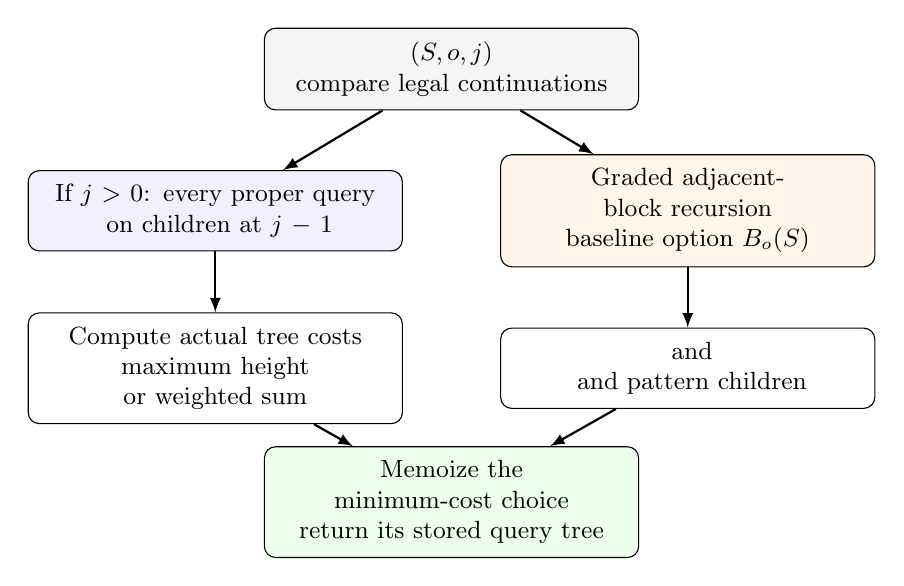
\begin{tikzpicture}[every node/.style={font=\small},
  box/.style={draw,rounded corners,align=center,inner sep=5pt,text width=4.4cm},
  arr/.style={-latex,thick}]
  \node[box,fill=gray!8] (rollout) at (0,0)
    {\Rollout$(S,o,j)$\\compare legal continuations};
  \node[box,fill=blue!6] (split) at (-3,-1.8)
    {If $j>0$: every proper query\\\Rollout\ on children at $j-1$};
  \node[box,fill=orange!8] (baseline) at (3,-1.8)
    {Graded adjacent-block recursion\\baseline option $B_o(S)$};
  \node[box] (grade) at (3,-3.8)
    {\HullData\ and \GradeDP\\\EndpointCode\ and pattern children};
  \node[box] (evaluate) at (-3,-3.8)
    {Compute actual tree costs\\maximum height or weighted sum};
  \node[box,fill=green!7] (best) at (0,-5.5)
    {Memoize the minimum-cost choice\\return its stored query tree};
  \draw[arr] (rollout) -- (split);
  \draw[arr] (rollout) -- (baseline);
  \draw[arr] (baseline) -- (grade);
  \draw[arr] (split) -- (evaluate);
  \draw[arr] (grade) -- (best);
  \draw[arr] (evaluate) -- (best);
\end{tikzpicture}
\caption{Exact lookahead wrapped around the quasipolynomial baseline.
The arrows denote calls and the returned trees or costs. The baseline
may end lookahead early at any reached state. The logarithmic cap on
$j$ bounds the number of reachable transcripts; it does not truncate
the completed identification tree. The proof compares this finite
search with an optimal tree, but the search evaluates only constructed
trees.}
\label{fig:qp-procedure-flow}
\end{figure}


\begin{theorem}\label{thm:qp-two-plus-epsilon}
For every fixed rational $\varepsilon>0$, both maximum depth and
arbitrary-prior expected depth admit quasipolynomial-time
$(2+\varepsilon)$ approximations using only supplied binary line
queries. For $0<\varepsilon\le1$, the running time is
$(mn)^{O(\varepsilon^{-1}\log n)}$ times a polynomial in the input
bit length. This scheme approaches factor two.
\end{theorem}
\begin{proof}
For $0<\varepsilon\le1$, take $\lambda=1+\varepsilon/2$ and
$a=2\lambda=2+\varepsilon$ in the two baseline constructions.
Their additive bounds imply the hypotheses of
Lemma~\ref{lem:lookahead-completion} with
\[
 L_W=\gamma\log_2n,\qquad L_E=c\ln n,
\]
because $\log_2|S'|\le\log_2n$ and
$\mathcal E(S')\le w(S')\ln n$. Choose the corresponding lookahead
length from that lemma. For $\varepsilon>1$, run the construction
with $\varepsilon=1$.

For implementation, choose fixed rational upper bounds on $\gamma$
and $c$, and replace logarithms in the lookahead lengths by
$\lceil\log_2 n\rceil$, which also upper-bounds $\ln n$.
Cap $k$ at $n-1$ if necessary; that permits every proper tree and
returns the exact optimum. The lookahead depth is $O(\log n)$
because $a-1\ge1$. At most $(2m)^{O(k)}$ states are reachable,
since each is determined by at most $k$ supplied query answers.
Each baseline call has $(mn)^{O(\varepsilon^{-1}\log n)}$ cost:
there are $O(\varepsilon^{-1}\log n)$ schedule grades, and their
counts and last positions have polynomial ranges. Multiplying the
two bounds gives the stated running time. Powers of rational
$\lambda$, count
capacities, and original prior weights have polynomial bit length
for fixed $\varepsilon$; the optimized objectives are rational
sums of actual tree costs. Thus no irrational comparisons are
required in the dynamic programs.
Every retained query properly splits its state, so the reconstructed
tree has at most $n$ leaves and $n-1$ internal nodes.
\end{proof}
